	\begin{center}
		\section{常用技巧（卡常，对拍，打表，调试等）}
	\end{center}

	\begin{multicols*}{2}

		\subsection{快读快写}
		下面这个模板来自 wida 的 GitHub 仓库并补充了一些功能，适合需要高性能读写的场景。

		\begin{minted}{cpp}
// 来自wida github仓库 https://github.com/hh2048/XCPC/tree/main 加了一些新功能
//46 ms https://acm.hdu.edu.cn/contest/view-code?cid=1179&rid=14912 读入字符getc(a) 的AC记录
// AC https://vjudge.net/solution/63197697 一道测试读写的codechef题目
namespace QuickRead {
	// 快读
	char buf[1 << 21], *p1 = buf, *p2 = buf;

	inline int getc() {
		return p1 == p2 && (p2 = (p1 = buf) + fread(buf, 1, 1 << 21, stdin), p1 == p2) ? EOF : *p1++;
	}

	template<typename T>
	void Cin(T &a) {
		T ans = 0;
		bool f = 0;
		char c = getc();
		for (; c < '0' || c > '9'; c = getc()) {
			if (c == '-') f = 1;
		}
		for (; c >= '0' && c <= '9'; c = getc()) {
			ans = ans * 10 + c - '0';
		}
		a = f ? -ans : ans;
	}

	void getc(char &a) {
		char c = getc();
		while (isspace(c)) {
			c = getc();
		}
		a = c;
	}

	template<typename T, typename... Args>
	void Cin(T &a, Args &... args) {
		Cin(a), Cin(args...);
	}

	// ===== 输出 =====
	static constexpr size_t OUT_CAP = 1 << 21; // 大概是2MB
	char obuf[OUT_CAP];
	size_t op = 0;

	inline void flush() {
		if (op) {
			fwrite(obuf, 1, op, stdout);
			op = 0;
		}
	}

	inline void putc(char c) {
		if (op == OUT_CAP) flush();
		obuf[op++] = c;
	}

	template<typename T>
	void write(T x) {
		// 注意，这里输出不带换行
		if (x < 0) putc('-'), x = -x;
		if (x > 9) write(x / 10);
		putc(x % 10 + '0');
	}

	struct Flusher {
		// 析构时自动刷新
		~Flusher() { flush(); }
	} flusher;
} // namespace QuickRead
using namespace QuickRead;
		\end{minted}

		\subsubsection{读入，输出科学计数法小数}

		正常来说是用不到这个东西的。

		\begin{minted}{cpp}
	// https://www.luogu.com.cn/record/230330447 科学计数法小数
	template<typename T>
	void Cinf(T &a) {
		// 新增：读取浮点数，支持科学计数法
		T ans = 0;
		bool f = 0; // 负号
		char c = getc();
		// 跳过非数字和小数点前的空白/符号
		while ((c < '0' || c > '9') && c != '.') {
			if (c == '-') f = 1;
			c = getc();
		}
		// 读取整数部分
		while (c >= '0' && c <= '9') {
			ans = ans * 10 + (c - '0');
			c = getc();
		}
		// 如果有小数点，读取小数部分
		if (c == '.') {
			c = getc();
			T frac = static_cast<T>(1);
			while (c >= '0' && c <= '9') {
				frac /= 10;
				ans += (c - '0') * frac;
				c = getc();
			}
		}
		a = f ? -ans : ans;
		// 处理科学计数法部分
		if (c == 'E' || c == 'e') {
			c = getc();
			bool exp_neg = false;
			if (c == '+') {
				c = getc();
			} else if (c == '-') {
				exp_neg = true;
				c = getc();
			}
			int exp = 0;
			while (c >= '0' && c <= '9') {
				exp = exp * 10 + (c - '0');
				c = getc();
			}
			T multiplier = pow(10.0, exp_neg ? -exp : exp);
			a *= multiplier;
		}
	}

	template<typename T>
	void writef(T x) {
		// 新增：输出浮点数，默认输出6位小数，支持四舍五入
		if (x < 0) putchar('-'), x = -x;
		using ll = long long;
		int prec = 6; // 默认精度6，可根据需要调整
		// 添加圆整因子
		T round_add = static_cast<T>(5);
		for (int i = 0; i < prec + 1; ++i) {
			round_add /= 10;
		}
		x += round_add;
		ll int_part = static_cast<ll>(x);
		write(int_part); // 输出整数部分
		putchar('.');
		T frac_part = x - int_part;
		for (int i = 0; i < prec; ++i) {
			frac_part *= 10;
			int digit = static_cast<int>(frac_part);
			putchar(digit + '0');
			frac_part -= digit;
		}
	}
		\end{minted}

		\subsection{开大栈空间}
		\href{https://acm.hdu.edu.cn/contest/clarification?cid=1198&tid=24339}{如何开大栈空间}

		正常应该是不需要选手去干这件事情的。

		杭电 OJ 暂不支持调整栈空间大小。如果使用 G++ 提交代码，且代码中递归层数较深，可能会返回 \texttt{Runtime Error (STACK\_OVERFLOW)}。可以在 \texttt{main()} 开头加入内联汇编手动切换到更大的栈空间。注意必须用 \texttt{exit(0)} 退出，不能 \texttt{return}，否则会访问已失效的旧栈帧。

		\textbf{x86\_64（Codeforces、洛谷、AtCoder 等绝大多数 OJ）：}

		\begin{minted}{cpp}
int main() {
    int size(256 << 20);  // 256M
    __asm__ volatile("movq %0, %%rsp" :: "r"((char *)malloc(size) + size));

    // 关同步流代码
    // 主程序代码

    exit(0);
}
		\end{minted}

		\textbf{AArch64 / ARM64（Apple Silicon 本地调试等）：}

		\begin{minted}{cpp}
int main() {
    int size(256 << 20);  // 256M
    asm volatile("mov sp, %0" :: "r"((char *)malloc(size) + size));

    // 关同步流代码
    // 主程序代码

    exit(0);
}
		\end{minted}

		\subsection{C++ 中 \texttt{struct} 自定义比较器 与 \texttt{std::array} 性能对比}
		在作为 \texttt{std::set} 和 \texttt{std::priority\_queue} 的元素时，使用自定义的 \texttt{struct}（配合自定义比较器）通常比使用 \texttt{std::array} （无论是自定义比较器还是默认比较器）具有更好的性能。
		根据基准测试，在 \texttt{std::set} 中，\texttt{struct} 的操作耗时比 \texttt{std::array} 显著更少（快约 30\% 到 50\%）。在 \texttt{std::priority\_queue} 中两者性能相近，但整体上 \texttt{priority\_queue} 远快于 \texttt{set}。因此，在对常数要求较高的题目中，建议使用 \texttt{struct} 替代 \texttt{std::array} 或 \texttt{std::tuple}，并优先考虑使用 \texttt{priority\_queue}。

		\href{https://gist.github.com/znzryb/bfc064b51520410569d562619ac0af11}{详细的基准测试代码与输出结果记录(gist 链接)}。

		\subsection{计时}
		\begin{minted}{cpp}
#include <chrono>
#include <iostream>

int main() {
    auto start = std::chrono::high_resolution_clock::now();

    // ... 你的代码 ...

    auto end = std::chrono::high_resolution_clock::now();

    // 转换为毫秒
    auto duration = std::chrono::duration_cast<std::chrono::milliseconds>(end - start);
    std::cout << "耗时: " << duration.count() << " ms\n";

    // 转换为微秒
    auto us = std::chrono::duration_cast<std::chrono::microseconds>(end - start);
    std::cout << "耗时: " << us.count() << " us\n";

    // 或者直接用浮点数秒
    std::chrono::duration<double> sec = end - start;
    std::cout << "耗时: " << sec.count() << " s\n";
}
		\end{minted}

		\subsection{对拍}

		对拍程序大致框架（windows）（不写 \texttt{.exe} 也是可以的）

		\begin{minted}{cpp}
#include <bits/stdc++.h>

int main() {
  // For Windows
  // 对拍时不开文件输入输出
  // 当然，这段程序也可以改写成批处理的形式
  while (true) {
    system("gen > test.in");  // 数据生成器将生成数据写入输入文件
    system("mySol.exe < test.in > a.out");  // 获取程序1输出
    system("std.exe < test.in > b.out");  // 获取程序2输出
    if (system("fc a.out b.out")) {
      // 该行语句比对输入输出
      // fc返回0时表示输出一致，否则表示有不同处
      system("pause");  // 方便查看不同处
      return 0;
      // 该输入数据已经存放在test.in文件中，可以直接利用进行调试
    }
  }
}
		\end{minted}

		\begin{center}
			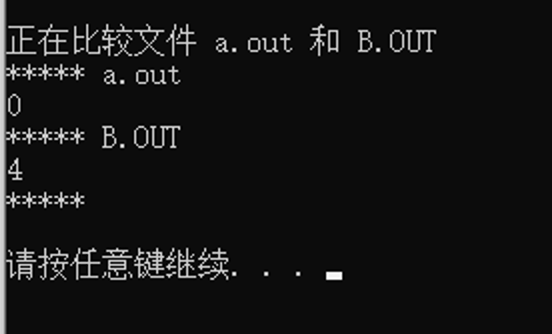
\includegraphics[width=\linewidth]{image/duipai_fc_output.png}
		\end{center}

		\texttt{fc} 函数的输出结果如上。

		Linux 可以像下面这么写。（其实就是把 \texttt{fc} 改成了 \texttt{diff}，其他其实差不太多）

		\begin{minted}{cpp}
#include <bits/stdc++.h>

using namespace std;

int main() {
    // 对拍时不开文件输入输出
    // 当然，这段程序也可以改写成批处理的形式
    int idx=0;
    while (true) {
        cerr<<"running on "<<++idx<<" test"<<"\n";
        // 下面的这些都是可执行程序
        // （相对）路径也是以这个可执行程序位置为准
        system("./D2_Tree_Orientation_Gen > test.in");  // 数据生成器将生成数据写入输入文件
        system("./D2_Tree_Orientation_Hard_Version < test.in > a.out");  // 获取希望检验输出
        system("./D1_Tree_Orientation_Easy_Version < test.in > b.out");  // 获取暴力程序输出
        if (system("diff a.out b.out")) {
            // 该行语句比对输入输出
            return 0;
            // 该输入数据已经存放在test.in文件中，可以直接利用进行调试
        }
    }
}
		\end{minted}

		\begin{center}
			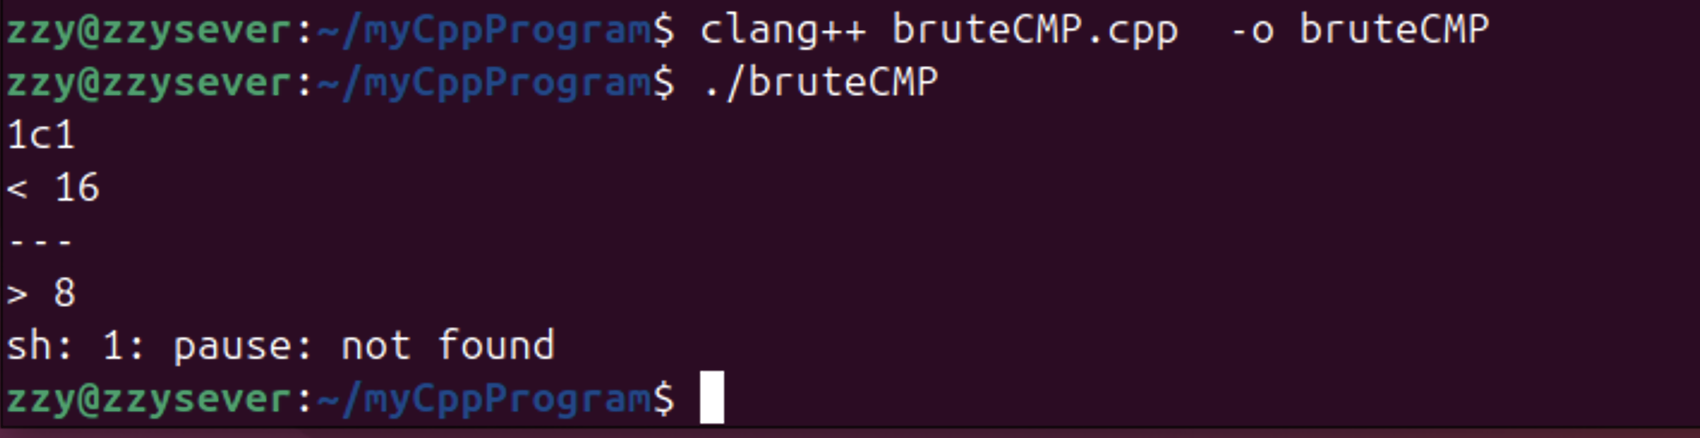
\includegraphics[width=\linewidth]{image/duipai_diff_output.png}
		\end{center}

		\subsection{打表}

		用 \texttt{system()} 调用编译好的生成器和暴力程序，批量跑数据并输出结果，方便观察规律。

		\begin{minted}{cpp}
struct Solve {
	// ll N;

	Solve() {
		// cin >> N;
		for (int i = 1; i <= 100; ++i) {
			system("./Good_Array_1_gen > in.txt");
			system("cat in.txt");
			system("./Good_Array_1__brute < in.txt > out.txt");
			cout << "\n"; // 这里需要加一个换行，才能更好地看清 out.txt
			system("cat out.txt");
			cout << "\n---------------\n";
		}
	}
};
		\end{minted}

		\textbf{Windows 注意}：Windows 下没有 \texttt{cat} 命令，需要换成 \texttt{type}。

		重定向 \texttt{cerr} 到文件：如果程序的输出走的是 \texttt{cerr}（比如调试信息），普通的 \texttt{>} 只能捕获 \texttt{stdout}。需要用 \texttt{2>} 或 \texttt{2>\&1} 进行重定向：

		\begin{minted}{bash}
# 只捕获 cerr（stderr）到 out.txt
./brute < in.txt 2> out.txt

# 同时捕获 cout（stdout）和 cerr（stderr）到 out.txt
./brute < in.txt > out.txt 2>&1
		\end{minted}

		不过一般我们只需要在\texttt{brute.cpp} 中在 \texttt{cerr} 输出调试信息，所以不需要这个。

		重定向后，\textbf{被重定向的流就不会再实时显示在终端里，而是写入文件}。比如用了 \texttt{2> out.txt} 之后，\texttt{cerr} 会消失在终端；用了 \texttt{> out.txt 2>\&1} 之后，\texttt{cout} 和 \texttt{cerr} 都会消失在终端。

		这里为什么不直接用\texttt{brute.cpp} 程序的标准输出流，而是写入文件？因为如果直接用标准输出流，那么 \texttt{brute.cpp} 的输出和这个 \texttt{in.txt} 的 \texttt{cat} 输出会混在一起，不方便观察。

		\subsubsection{打表中需要输出的东西（答案）}
		\href{https://www.codechef.com/problems/BINCON}{Binary Construction} 这个是一道典型的打表题目，只需要使用暴力输出答案，即可一眼看出规律。

		\begin{minted}{text}
1
01
011
1001
10001
100001
1000001
.......
10000000000001
100000000000001
1000000000000001
10000000000000001
		\end{minted}

		但是，由于我们采用了放弃大脑思考，以对拍代替大脑思考的策略，显然，我们不止在打表题目进行打表，而是在很多题目上都打表，那么如何打表才能够更好地观察规律，找到解法，帮助我们解决问题呢？

		\subsubsection{打表中需要输出的东西（前缀答案）}

		\href{https://www.codechef.com/problems/GOOD1}{Good Array 1} 输出前缀答案，可以帮助我们看出来这道题目是不是前缀 dp。

		\begin{minted}[highlightlines={4,13}]{text}
	
1
8
2 7 1 4 6 6 4 4 
[dp] = [0, 0, 0, 0, 0, 1, 1, 2]

*************************
2

*************************
1
7
4 3 3 1 4 5 6 
[dp] = [0, 0, 1, 1, 1, 1, 1]

*************************
1

		\end{minted}

		不过其实不是每道题目都是适合这个打表的，对于一些题目，头脑风暴或者其他方法可能更加适合。

		\subsection{凸包数据生成}

		对拍几何题（凸包、旋转卡壳、闵可夫斯基和等）需要快速生成 CCW 序凸多边形。每次随机选椭圆长短轴比 $\in [1, 3]$ + 随机旋转角，覆盖近圆 / 椭圆 / 倾斜椭圆等曲率非均匀形状（破除「近圆形 monotonicity 盲区」），然后随机 $N$ 个角度排序映射上去。\texttt{T} 模板参数：\texttt{T = ll} 走 \texttt{llround} 钉整数（题面整数坐标）、\texttt{T = DB} 保留 cos/sin 原浮点（精度/边界更细）；坐标范围 $x, y \in [-R, R]$（椭圆 $R \cos \theta$、$\tfrac{R}{\text{asp}}\sin \theta$ 内嵌半径 $R$ 圆盘，旋转 $\varphi$ 不变半径，\texttt{llround} 边界 $\pm 1$ 不溢出）。\texttt{allow\_collinear} 切换严格凸（cross $> 0$）和允许三点共线（cross $\ge 0$，但仍要求至少一处真左转保证多边形面积非零）。可行域实测：$R = 10^9$ 时 $N \le 2000$ 安全（$N = 5000$ 严格模式 75\,\% 失败）；$N/R \gtrsim 0.3$ 严格模式 retry 显著上升、$\gtrsim 0.5$ 不可行（如 $R = 100$、$N = 50$ 100\,\% 卡死）。要求 $N \ge 3$，超出可行域时自旋等死（外面套 retry 上限自己加）。

		\begin{minted}{cpp}
mt19937_64 rng(chrono::steady_clock::now().time_since_epoch().count());

// T = ll : 整数坐标（llround）   /   T = DB : 浮点坐标（保留原值）
// 坐标范围 |x|, |y| <= R
template<class T>
vector<Point<T>> gen_convex_polygon(int N, bool allow_collinear = false,
                                    ll R = 1'000'000'000) {
    // 退化 case (N <= 2): 主循环对 N <= 2 必死循环
    // (N=1: j=(0+1)%1=0=i, A[i]==A[j] 永真; N=2: k=(0+2)%2=0=i, cross 三点退化恒 0).
    // 直接撒 N 个不重点返回, 跳过 CCW 校验.
    if (N <= 2) {
        set<pair<T, T>> S;
        while ((int) S.size() < N) {
            if constexpr (is_floating_point_v<T>) {
                S.insert({uniform_real_distribution<T>(-(T) R, (T) R)(rng),
                          uniform_real_distribution<T>(-(T) R, (T) R)(rng)});
            } else {
                S.insert({uniform_int_distribution<T>(-(T) R, (T) R)(rng),
                          uniform_int_distribution<T>(-(T) R, (T) R)(rng)});
            }
        }
        vector<Point<T>> A;
        for (auto [x, y] : S) A.push_back(Point<T>(x, y));
        return A;
    }
    DB phi = uniform_real_distribution<DB>(0, 2 * M_PI)(rng);
    DB asp = uniform_real_distribution<DB>(1.0, 3.0)(rng); // 1=圆, >1=椭圆
    DB cp = cos(phi), sp = sin(phi);
    while (true) {
        vector<DB> th(N);
        for (auto& t : th) t = uniform_real_distribution<DB>(0, 2 * M_PI)(rng);
        sort(th.begin(), th.end());
        vector<Point<T>> A(N);
        for (int i = 0; i < N; ++i) {
            DB x = R * cos(th[i]), y = R / asp * sin(th[i]);  // 椭圆
            DB rx = cp * x - sp * y, ry = sp * x + cp * y;    // 旋转 phi
            if constexpr (is_floating_point_v<T>) {
                A[i] = Point<T>(rx, ry);
            } else {
                A[i] = Point<T>((T) llround(rx), (T) llround(ry));
            }
        }
        bool ok = true, has_turn = false; // has_turn: 至少一处真左转
        for (int i = 0; i < N && ok; ++i) {
            int j = (i + 1) % N, k = (i + 2) % N;
            if (A[i] == A[j]) { ok = false; break; }
            auto c = cross(A[i], A[j], A[k]);
            if (allow_collinear ? c < 0 : c <= 0) { ok = false; break; }
            if (c > 0) has_turn = true;
        }
        // allow_collinear 下若全程 cross == 0 则点全共线、面积 = 0，得重抽
        if (ok && !has_turn) ok = false;
        if (ok) return A;
    }
}
		\end{minted}

		\subsection{编译 shell}

		\begin{minted}{bash}
clang++ "$1" && ./a.out
		\end{minted}

		\begin{center}
			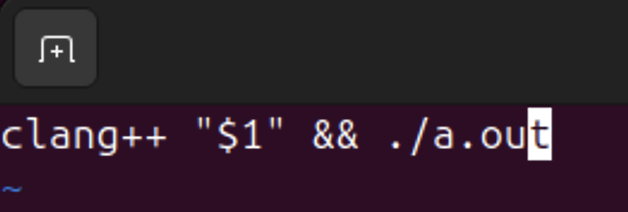
\includegraphics[width=\linewidth]{image/compile_shell_usage_1.png}
		\end{center}

		\begin{center}
			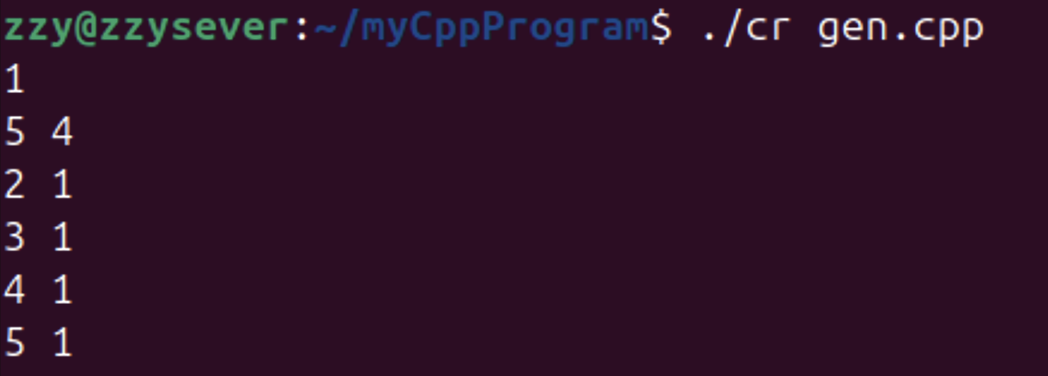
\includegraphics[width=\linewidth]{image/compile_shell_usage_2.png}
		\end{center}

	\end{multicols*}

